\documentclass {article}
\usepackage{graphicx}
\usepackage{fullpage}
%\usepackage{amsmath}
\usepackage{color}
\usepackage{fancyvrb}
\usepackage{parskip} % provides for indentless-but-spaced paragraphs
\usepackage[usenames,dvipsnames]{xcolor}
\usepackage{paralist}
\usepackage{minted}
\begin {document}

\title{Domain-blind validation of Big Data}

\maketitle

\tableofcontents

\section{Overview}
\subsection{What \emph{is} it?}
BDQC is a Python 3\footnote{https://wiki.python.org/moin/Python2orPython3}
software framework and executable module.
Although it provides built-in capabilities that make it useful
``out of the box'', being a ``framework'' means that users (knowledgeable
in Python programming) can extend its capabilities, and it is designed to
be so extended.

\subsection{What is it \emph{for}?}
{\bf BDQC identifies anomalous files among large collections of files which are
\emph{a priori} assumed to be ``similar.''}
It is intended to:
\begin{enumerate}
\item validate primary input data.
\item validate output (or intermediate stages of) data processing pipelines.
\item discover potentially ``interesting'' outliers.
\end{enumerate}
These use cases merely highlight different sources of anomalies in data.
In the first, anomalies might be due to faulty data handling or acquisition
(e.g. sloppy manual procedures or faulty sensors). In the second, anomalies
might appear in data due to bugs in pipeline software or runtime failures
(e.g. power outages, network unavailablity, etc.). Finally, anomalies that
can't be discounted as being due to technical problems might actually be
``interesting'' observations to be followed up in research.
% In other words, although it was developed as a rapid means of spotting
% problems in pipelines (``validating'' or ``QC'ing'' data), it can serve
% the goal of discovery as well.

Although it was developed in the context of genomics research, it is 
expressly not tied to a specific knowledge domain. It can, however,
be customized (via the plugin mechanism) for specific knowledge domains.
% motivated by realization that when faced with thousands of individual
% files it becomes challenging to even confirm they all contain approximately
% "what they should."

Importantly, \emph{files} are its fundamental unit of operation.
This means that a file must constitute a meaningful unit of
information---one sample's data, for example---in any application of BDQC. % (for \#3 above to be well-defined).

\subsection{What does it \emph{do}?}

BDQC analyzes a collection of files in two stages.
First, it analyzes each file individually and produces a summary of the
file's content (\emph{within-file} analysis). Second, the summaries are
aggregated, and the aggregate data is analyzed (\emph{across-file}
analysis). The exhaustive aggregate analysis is saved to a (JSON) file,
and anomalous files---that is, files that are outliers in one or more
statistics---are summarized along with the evidence in an HTML report. 

BDQC can be run from the command line and command line arguments control
which files are analyzed,
how individual files are analyzed,
how the aggregate file analyses are analyzed.
All command line arguments are optional; the framework will carry out
default actions. See command line help.

Alternatively, the bdqc.Executor Python class can be incorporated directly
into third party Python code. This allows it to be incorporated into
pipelines.

\subsection{How does it work?}
\subsubsection{Stage 1 --- Summary production}

The BDQC \emph{framework} orchestrates the execution of \emph{plugins}.
{\bf All of the within-file analysis capabilities are provided by
plugins}\footnote{The BDQC \emph{package} includes several
``built-in'' plugins which allow it to be useful ``out of the box.''}.
That is, the plugins that are executed on a file entirely determine the
content of the summary generated for that file.
The framework:
\begin{enumerate}
\item assembles a list of paths identifying files to be analyzed
\item executes a specified set (actually a directed acyclic graph (DAG))
		of plugins on each filename
\item manages the aggregation of plugins' results into a summary for each file,
\item and performs the final aggregate analysis.
\end{enumerate}

Plugins exist in a DAG because each plugin can declare (as part of its
implementation) zero or more dependencies. The framework insures that:
\begin{enumerate}
\item dependencies of Plugin \emph{P} are executed before \emph{P} is executed
\item each plugin is provided with the results of the plugins on which it
	depends
\end{enumerate}

The framework minimizes work by only executing a plugin when required.

Again, the BDQC \emph{framework} does not touch files' content---it only handles
filenames.
\subsubsection{Stage 2 --- Summary analysis}
but it does perform all the \emph{aggregate} analysis.
The aggregate analysis consists of a set statistical techniques to
identify outliers in the \emph{univariate} statistics produced by plugins.
By default, any file that is an outlier in any statistic is flagged as
potentially anomalous.
The framework identifies univariate statistics in the plugins' results
and selects statistical tests according to types of the statistics
(quantitative, ordinal or categorical).

%Requiring all file analysis to reside in plugins insures maximum
%extensibility. Moreover, this architecture is intended to motivate quality
%coding and maximize reuse. A plugin should ideally perform a single
%well-defined analysis, making it simple to unit test.

{\centering
\begin{figure}[h]
\includegraphics[scale=0.8]{dataflow}
\end{figure}
}

\subsection{Design goals}
The BDQC framework was developed with several explicit goals in mind:
\begin{enumerate}
\item Identify an ``anomalous'' file among a large collection of
	\emph{similar} files of \emph{arbitrary} type
	with as little guidance from the user as possible, ideally none.
	In other words, it should be useful ``out of the box'' with almost no
	learning curve.
\item ``Simple things should be simple; complex things should be
	possible\footnote{Alan Kay}.''
	Although basic use should involve almost no learning curve, it should
	be possible to extend it with arbitrarily complex (and possibly
	domain-specific) analysis capabilities.
\item Plugins should be simple (for a competent Python programmer) to
	develop, and the system must be robust to faults in plugins.
\end{enumerate}

The third goal motivated the use of Python.

\section{Installation}

The BDQC framework has no requirements other than Python 3.3.2 or later.
After extracting the archive...

{\tt python3 setup.py install}

...installs the framework, after which...

{\tt python3 -m bdqc.scan <directory> }

...will analyze all files in {\tt <directory>}, and
{\tt python3 -m bdqc.scan --help} provides further help.
The contents of the online help is not repeated in this document.


\newpage
\section{Plugins}
To reiterate, the BDQC executable \emph{framework} does not touch
files itself. All file analysis is carried out by plugins,
several of which are included in but, nonetheless, distinct from the
framework. 

A plugin is simply a Python module with several required and optional
elements shown in the example below.

\begin{minted}{python}
VERSION=0x00010000
DEPENDENCIES = ['bdqc.builtin.extrinsic','some.other.plugin']
def process( filename, dependencies_results ):
	# Whatever processing is required to compute the values
	# x, [3,"ABC",5.532], and "yes", returned below.
	return {'a_statistic':x, 'another_result':[3,"ABC",5.532],
   		'a_final_result':"yes" }
\end{minted}

As shown in the example:
\begin{enumerate}
\item Every plugin \emph{must} provide a list called DEPENDENCIES (which may be empty).
	Each dependency is a fully-qualified Python package name.
\item Every plugin \emph{must} provide a two-argument function called process.
\item The process function \emph{must} return a Python dict or None.
\item The VERSION number is optional. If it is present:
	\begin{enumerate}
	\item it is included in output results
	\item it must be convertable to an integer (using int())
	\item it is used by the framework to decide whether to \emph{re}run a plugin
	\end{enumerate}
\item The returned dict \emph{may} contain anything, but see below.
\end{enumerate}

These requirements do not limit what a plugin can \emph{do}.
They merely define a \emph{packaging} that allows the plugin to be hosted
by the framework. In particular, a plugin may invoke compiled code (e.g.
C or Fortran) and/or use arbitrary 3rd party libraries using standard
Python mechanisms.

Although a plugin \emph{may} return effectively anything (containable in a
dict), the framework (currently) ignores in its final analysis non-scalar
values. Only scalar-valued statistics (quantitative, ordinal or
categorical) are incorporated in the cross-file analysis.

Moreover, while a plugin is free to return multiple statistics,
the Unix philosophy of ``Do one thing and do it well''\footnote{
https://en.wikipedia.org/wiki/Unix\_philosophy}
suggests it \emph{should} return only one.
This promotes unit-testability of plugins, and is the
motivation behind the plugin architecture.

There is no provision for passing arguments to plugins from the framework
itself.
Environment variables can be used when a plugin must be
parameterized.\footnote{One
use for set-valued returns is passing arguments to a ``downstream''
(depenendent) plugin.}

Developers are advised to look at the source code of any of the built-in
plugins for examples of how to write their own.
The {\tt bdqc.builtin.extrinsic} is a very simple plugin;
{\tt bdqc.builtin.tabular} is much more complex and demonstrates how
to use C code.
\newpage
\section{Framework execution}

After parsing command line arguments the framework ({\tt bdqc.scan}):
\begin{enumerate}
\item builds a list \(P\) of all candidate plugins
\item identifies an ordering of plugins that respects all declared
	dependencies
\item builds a list \(F\) of files to be (potentially) analyzed
\item for each file \(f\) in \(F\), for each plugin \(p\) in \(P\)
	it runs \(p\) on \(f\) \emph{if it needs to be run}
\end{enumerate}

The files to be analyzed as well as the set of candidate plugins are
controlled by multiple command line options. See online help.

These steps always happen.
Aggregate analysis---that is, analysis of the plugins' analyses---is
carried out if and only if a file is specified (with the {\tt --accum}
option) to contain the plugins' results.

Whether a plugin is actually run on a file depends on global options,
the existence of earlier analysis results, the modification time of
the file and the version (if present) of the plugin.

A plugin is run on a file:
\begin{enumerate}
\item if the {\tt --clobber} flag is included in the command line; this
	forces (re)run and preempts all other considerations.
\item if no results from the current plugin exist for the file.
\item if results exist but their modification time is older than the file.
\item if any of the plugin's dependencies were (re)run.
\item when the plugin version is (present and) newer (greater) than the
	version that produced existing results.
\end{enumerate}

\subsection{Built-ins}
The BDQC software package includes several built-in plugins so that it is
useful ``out of the box.'' These plugins provide very general purpose analyses
and assume \emph{nothing} about the files they analyze.
Although their output is demonstrably useful on its own, the built-in plugins
may be viewed as a means to ``bootstrap'' more specific (more domain-aware)
analyses.
\subsubsection{Extrinsic}
TODO
\subsubsection{Filetype}
TODO
\subsubsection{Tabular}
TODO

%Because it is intended to be be ``domain blind'' the analysis of a file
%proceeds heuristally.

%using a series of heuristics and
%produces a single file summarizing the analysis (in JSON format).

%Files can be specified in several ways including lists of directory trees
%to be search recursively or manifests. Additionally filters can be specified
%to refine the search.

%Extractors
%	all first-level scalars are taken by default +
%	any others specified
%
%Quantitative model-based (Gaussian) outlier detection
%Categorical
%	unanimity
%	conditional unanimity
%Ordinal
%	any missing value
%Set-valued
%	identity
%
%
%Scalar
%	Quantitative
%		robust outlier detection.
%	Categorical.
%		predefined rules
%			if >N% of values are identical, all should be
%			alert to any non-unanimity
%	Ordinal
%		essentially preclude outliers
%Multi-valued
%	Quantitative
%		categorical values
%			all
%
%Table analysis can be decomposed into
%	0. an upstream configuration requirement
%		"all categorical data to accumulate up to 23 labels (to capture chromosome)"
%	1. an extraction problem
%		"pull */tabledata/columns/labels out of all files' .bdqc"
%	2. an analysis
%		All sets should be identical

\end{document}

